% chapters/dp.tex

\chapter{Dynamic Programming}	\label{chapter:dp}

% file: algs/dp/binom-recursive.tex

\begin{algorithm}[H]
  \caption{Computing $\binom{n}{k}$.}
  \label{alg:binom-recursive}
  \begin{algorithmic}[1]
    \Procedure{Binom}{$n, k$} \Comment{Required: $n \ge k \ge 0$}
      \If{$k = 0 \lor n = k$}
	\State \Return 1
      \EndIf

      \State \Return $\Call{Binom}{n-1, k} + \Call{Binom}{n-1, k-1}$
    \EndProcedure
  \end{algorithmic}
\end{algorithm}



\begin{figure}[h]
  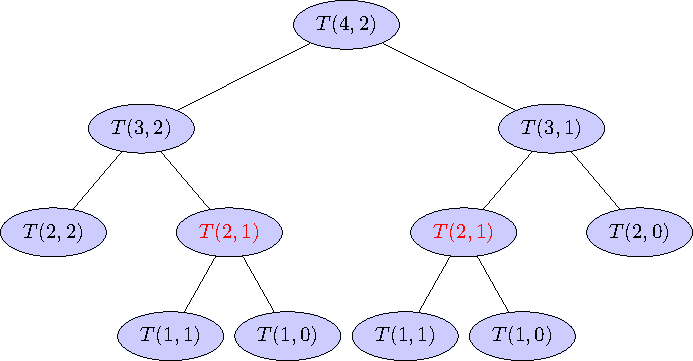
\includegraphics[width = 0.75\textwidth]{figs/binom-4-2}
  \caption{Calculate $\binom{4}{2}$ recursively.}
  \label{fig:binom-recursive}
\end{figure}

\begin{figure}[h]
  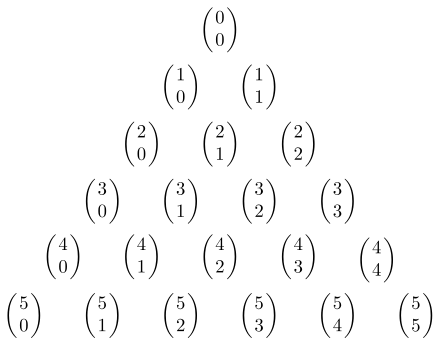
\includegraphics[width = 0.65\textwidth]{figs/pascal}
  \caption{Pascal triangle for binomial coefficients.}
  \label{fig:pascal}
\end{figure}

% file: algs/dp/binom-dp.tex

\begin{algorithm}[H]
  \caption{Computing $\binom{n}{k}$ by dynamic programming.}
  \begin{algorithmic}[1]
    \Procedure{Binom}{$n, k$} \Comment{Required: $n \ge k \ge 0$}
      \For{$i \gets 0 \;\text{\bf to}\; n-k$}
	\State $B[i][0] \gets 1$
      \EndFor

      \For{$i \gets 1 \;\text{\bf to}\; k$}
	\State $B[i][i] \gets 1$
      \EndFor

      \For{$j \gets 1 \;\text{\bf to}\; k$}
	\For{$d \gets 1 \;\text{\bf to}\; n-k$}
	  \State $i \gets j + d$
	  \State $B[i][j] \gets B[i-1][j] + B[i-1][j-1]$
	\EndFor
      \EndFor
      \State \Return $B[n][k]$
    \EndProcedure
  \end{algorithmic}
\end{algorithm}


\[
  (n-k+1) + (k) + k (n-k) = nk - k^2 + n + 1
\]

% file: algs/max-subarray-origin.tex

\begin{algorithm}[H]
  \caption{Max-sum subarray.}
  \label{mss-origin}
  \begin{algorithmic}[1]
    \Procedure{MSS}{$A[1 \cdots n]$}
      \State $\text{MSS}[0] \gets 0$

      \hStatex
      \For{$i \gets 1 \;\text{\bf to } n$}
	\State $\text{MSS}[i] \gets \max\left\{\text{MSS}[i-1] + A[i], 0\right\}$
      \EndFor

      \hStatex
      \State \Return $\max\limits_{1 \le i \le n} \text{MSS}[i]$
    \EndProcedure
  \end{algorithmic}
\end{algorithm}

% file: algs/max-subarray.tex

\begin{algorithm}[H]
  \caption{Max-sum subarray (Implementation Simplified).}
  \label{alg:mss}
  \begin{algorithmic}[1]
    \Procedure{MSS}{$A[1 \cdots n]$}
      \State $\text{mss} \gets 0$
      \State $\text{MSS} \gets 0$

      \hStatex
      \For{$i \gets 1 \;\text{\bf to } n$}
	\State $\text{MSS} \gets \max\left\{\text{MSS} + A[i], 0\right\}$
	\State $\text{mss} \gets \max\left\{\text{mss}, \text{MSS}\right\}$
      \EndFor

      \hStatex
      \State \Return $\text{mss}$
    \EndProcedure
  \end{algorithmic}
\end{algorithm}

